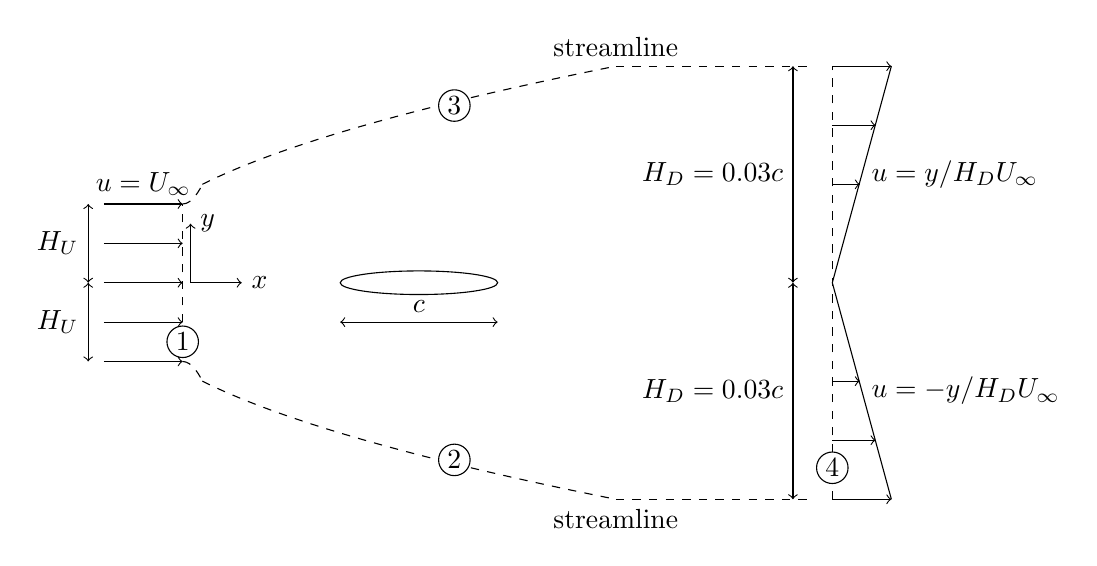
\begin{tikzpicture}
\foreach \x in {-2,-1,0,1,2} {
\draw[->] (0,\x/2) -- (1,\x/2);
}
\draw[<->] (-0.2,-1) -- (-0.2,0) node[midway,left] {$H_{U}$};
\draw[<->] (-0.2,1) -- (-0.2,0) node[midway,left] {$H_{U}$};
\node at (0.5,1.25) {$u=U_{\infty}$};
\draw[dashed] (1,-0.5) -- (1,1);
\draw (1,-0.75) circle (0.2cm);
\node at (1,-0.75) {$1$};
\draw[->] (1.1,0) -- (1.75,0) node[right] {$x$};
\draw[->] (1.1,0) -- (1.1,0.75) node[right] {$y$};
\draw[dashed] (1,1) parabola (1.25,1.25);
\draw[dashed] (1,-1) parabola (1.25,-1.25);
\draw[dashed] plot[smooth,domain=1:2] ({\x^2+0.25},\x+0.25);
\draw[dashed] plot[smooth,domain=1:2] ({\x^2+0.25},-\x-0.25);
\draw (4.45,2.25) circle (0.2cm);
\node at (4.45,2.25) {$3$};
\draw (4.45,-2.25) circle (0.2cm);
\node at (4.45,-2.25) {$2$};
\draw[dashed] plot[smooth,domain=2.1:2.5] ({\x^2+0.25},\x+0.25);
\draw[dashed] plot[smooth,domain=2.1:2.5] ({\x^2+0.25},-\x-0.25);
\draw[dashed] (6.5,2.75) -- (9,2.75);
\draw[dashed] (6.5,-2.75) -- (9,-2.75);
\draw[<->] (8.75,0) -- (8.75,2.75) node[midway,left] {$H_{D}=0.03c$};
\draw[<->] (8.75,0) -- (8.75,-2.75) node[midway,left] {$H_{D}=0.03c$};
\draw[dashed] (9.25,-2.15) -- (9.25,2.75);
\draw[dashed] (9.25,-2.75) -- (9.25,-2.55);
\draw (9.25,-2.35) circle (0.2cm);
\node at (9.25,-2.35) {$4$};
\draw (10,2.75) -- (9.25,0) node[midway,right] {$u=\brak{y/H_{D}}U_{\infty}$} -- (10,-2.75) node[midway,right] {$u=\brak{-y/H_{D}}U_{\infty}$};
\draw[->] (9.25,-2.75) -- (10,-2.75);
\draw[->] (9.25,-2) -- (9.8,-2);
\draw[->] (9.25,-1.25) -- (9.6,-1.25);
\draw[->] (9.25,2.75) -- (10,2.75);
\draw[->] (9.25,2) -- (9.8,2);
\draw[->] (9.25,1.25) -- (9.6,1.25);
\node at (6.5,3) {streamline};
\node at (6.5,-3) {streamline};
\draw[<->] (3,-0.5) -- (5,-0.5) node[midway,above] {$c$};
\draw (4,0) ellipse (1cm and 0.15cm);
\end{tikzpicture}